\chapter{Oktalno stablo}
\label{chapter:octree}

Oktalno stablo (\textit{Octree}) je struktura podataka kod koje svaki čvor stabla
ima točno 8 čvorova djece. Često se koristi u računalnoj grafici i geometriji,
jer omogućava jednostavnu rekurzivnu podjelu prostora na oktante. Primjenjuje se
u raznim algoritmima optimizacije geometrijskih operacija zbog velike efikasnosti. ~\cite{octree}

\begin{figure}[ht]
    \centering
    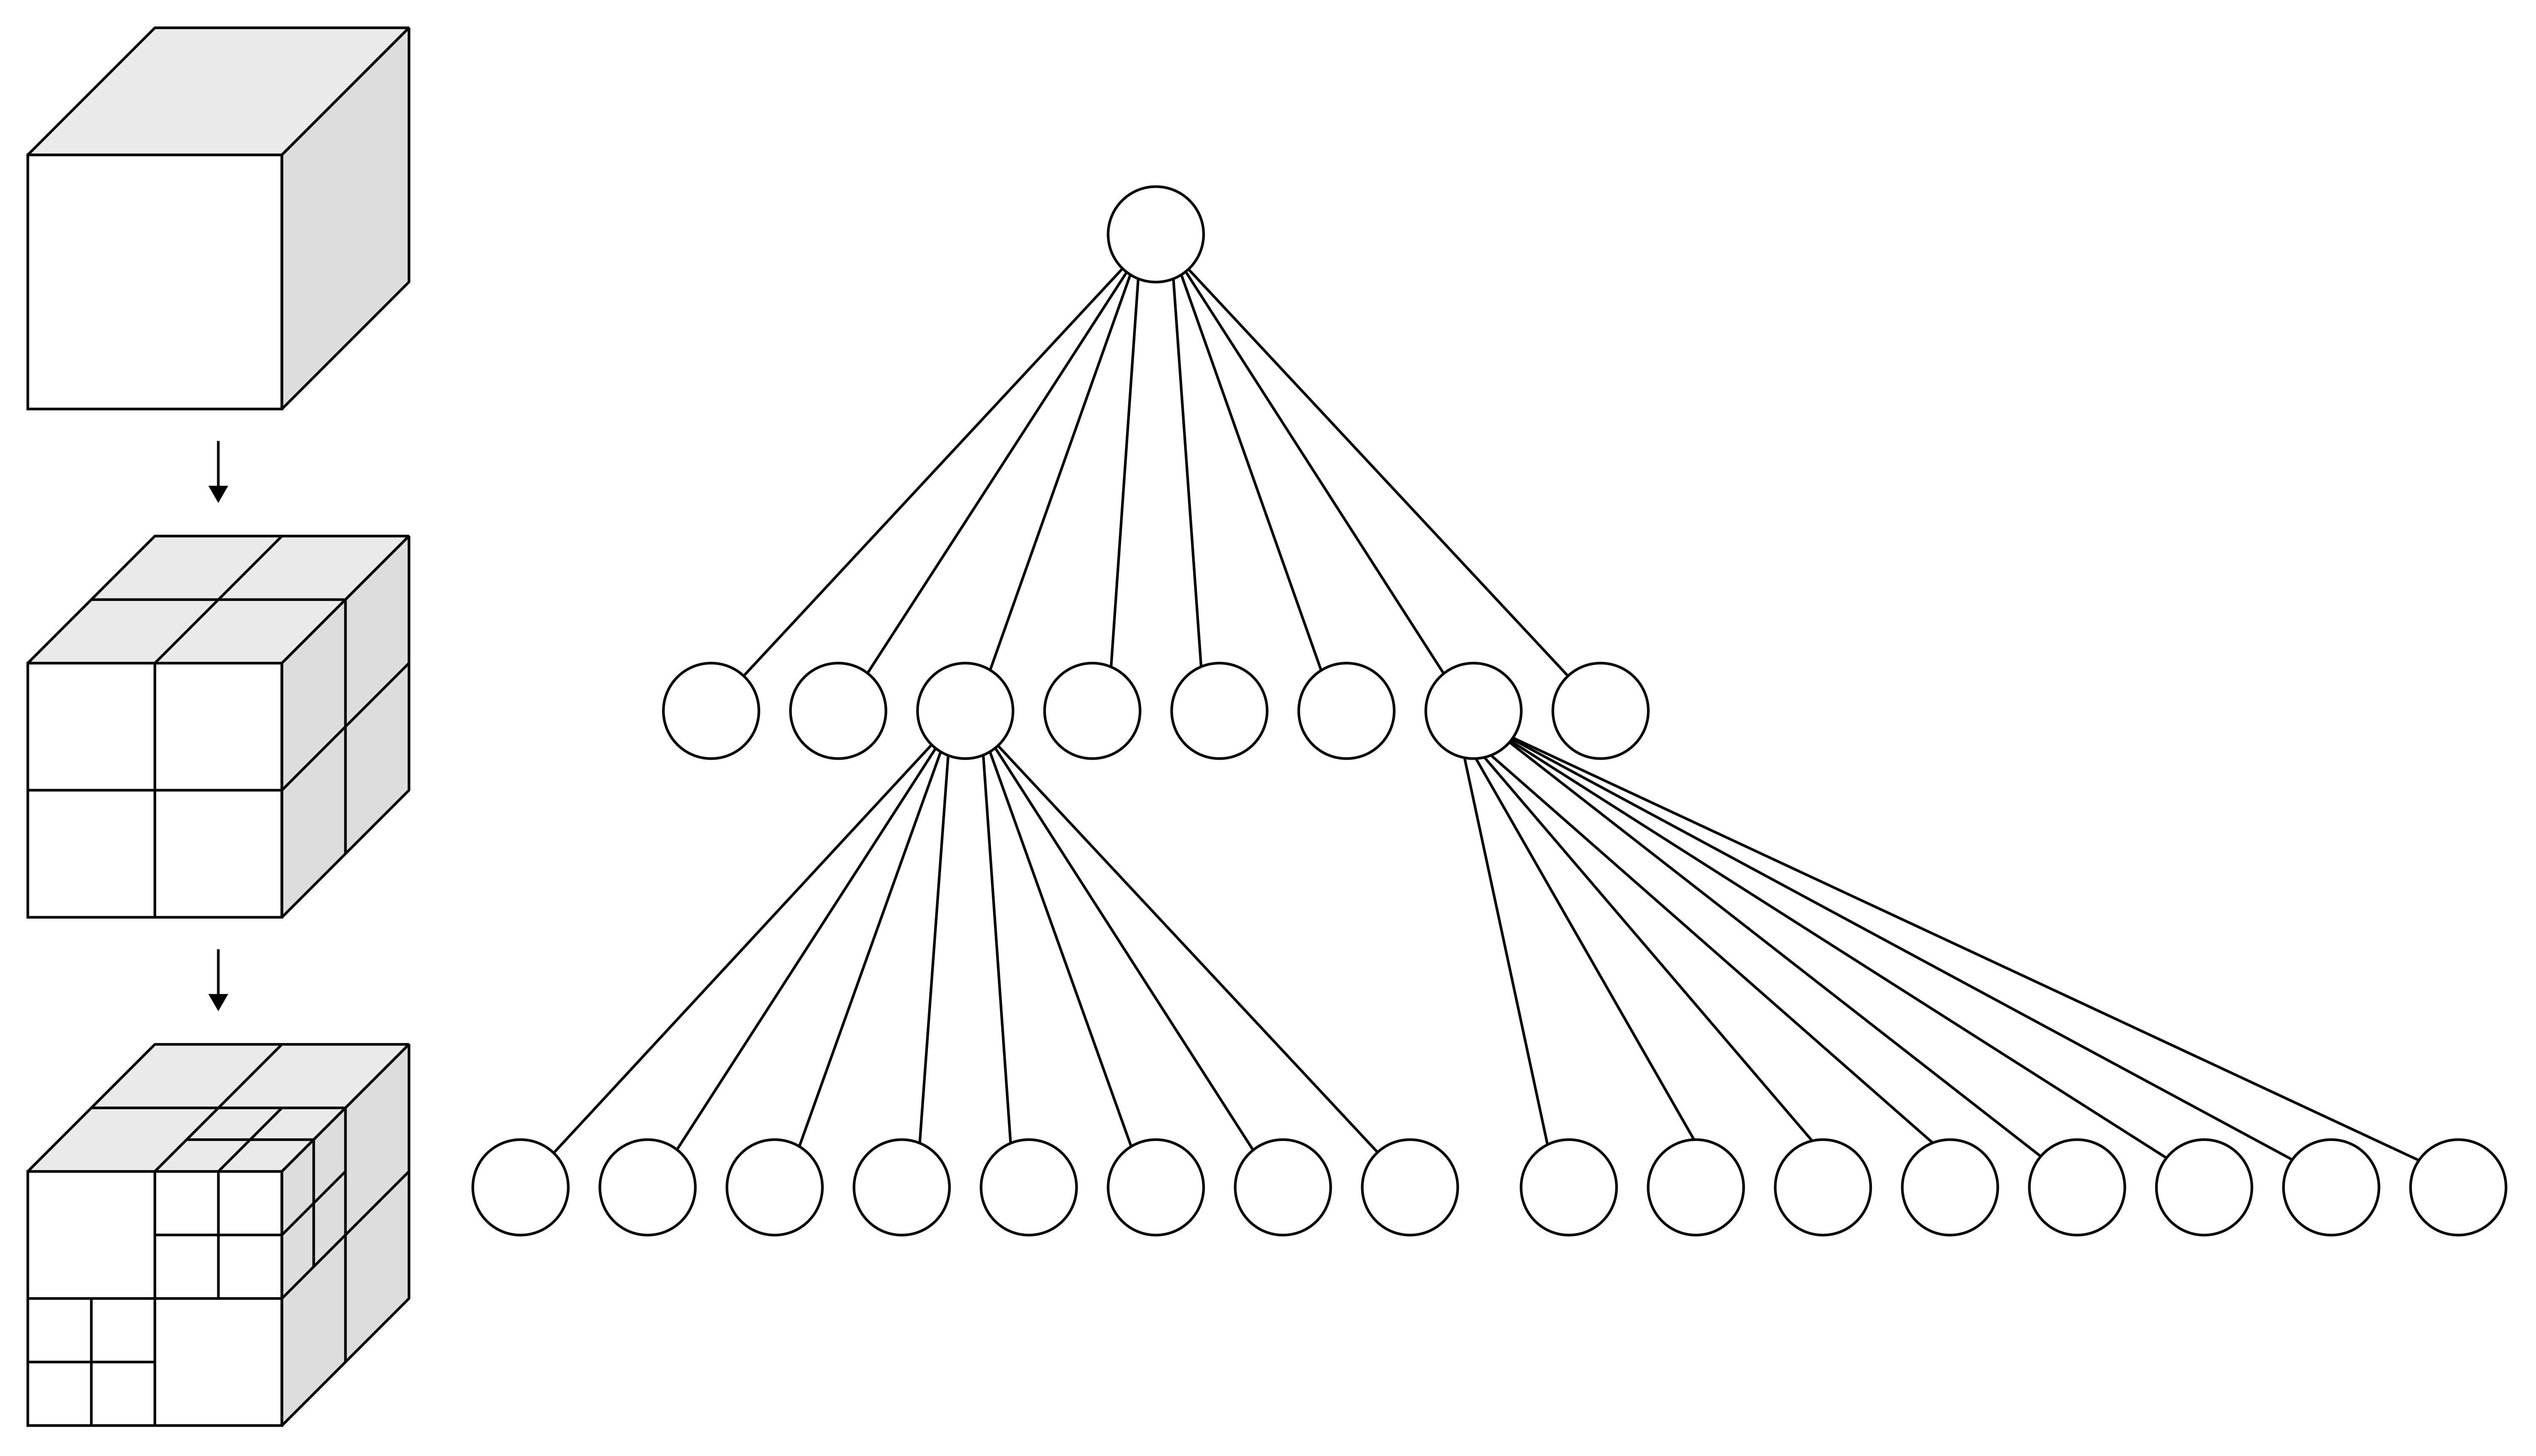
\includegraphics[width=15cm]{octree.png}
    \caption {Prikaz strukture oktalnog stabla}
\end{figure}

\section{Metode grananja}
\subsection{Potpuno oktalno stablo}

Potpuno oktalno stablo je podvrsta oktalnog stabla kod koje svaki unutarnji čvor
ima točno osam čvorova djece. Kod potpunog oktalnog stabla, broj čvorova na najnižoj razini
moguće je odrediti unaprijed kao
\[n_{razina} = 2^{3\cdot razina}\]

Nedostaci potpunog oktalnog stabla su veliko zauzeće memorije, kao i činjenica da će za većinu
modela nepravilnog oblika većina oktanata biti prazna.

\subsection{Grananje po potrebi}

Za razliku od potpunog oktalnog stabla, kod ovakvog tipa strukture čvorovi se granaju ovisno o zadanim
kriterijima, što će ponekad rezultirati neravnomjernom raspodjelom oktanata unutar stabla. Djelovi strukture
koji sadrže više primitivnih objekata granat će se na više razina, dok će oni djelovi koji imaju manje 
takvih objekata biti granani na manje razina.\\
Prednost ovakvog tipa strukture je puno manje zauzeće memorije i puno brža mogućnost pretrage, s obzirom
da velik broj čvorova nije potrebno provjeravati

\section{Primjena kod pronalaženja sudara}

Struktura oktalnog stabla implementirana je u ovom radu kao metoda optimizacije detekcije sudara dvaju trodimenzionalnih objekata.
Objekti nad kojima se vrši detekcija sudara su strukture predstavljene kao mreža trokuta, a učitavaju se iz \textit{Wavefront OBJ} datoteka.
Korišteno je grananje po potrebi (\textit{Branch-on-need}), a broj razina dubine stabla ograničen je na pet.
\pagebreak
\subsection{Parametri oktalnog stabla}

Svaki čvor oktalnog stabla opisan je sa 4 parametra koji su definirani kao članske varijable klase \textit{Octree}

\begin{enumerate}
  \item \textit{members} - svi primitivi (trokuti) koji se (dijelom ili potpuno) nalaze u tom čvoru stabla
  \item \textit{bounds} - objekt tipa \textit{BoundingBox} koji sadržava AABB (Axis-aligned bounding box)
  \item \textit{children} - niz od osam pokazivača na čvorove djecu
  \item \textit{level} - dubina u odnosu na korijenski čvor
\end{enumerate}

Kako bi se pojednostavnila implementacija, svaki od čvorova djece (razine veće od 0) sadrži i pokazivač na korijenski čvor.
\\\\
\textit{BoundingBox} je klasa koja definira strukturu tipa AABB (Axis-aligned bounding box). Koristi se na nultom čvoru za definiranje
kvadra koji opisuje 3D tijelo. Kod čvorova djece rekurzivno se dijeli do definiranih ograničenja, a opisuje prostor koji svaki od 
čvorova oktalnog stabla predstavlja.\\
Definiran je skupom od 8 točaka koji predstavljaju vrhove kvadra, te jednom točkom koja predstavlja njegov centar.
Indeksi vrhova određeni su prema pravilu tablice istinitosti.
\begin{center}
  \begin{tabular}{ c | c | c | c }
    \textbf{INDEX} & \textbf{RIGHT} & \textbf{TOP} & \textbf{FRONT} \\
    \hline
    0 & 0 & 0 & 0 \\
    1 & 0 & 0 & 1 \\
    2 & 0 & 1 & 0 \\
    3 & 0 & 1 & 1 \\
    4 & 1 & 0 & 0 \\
    5 & 1 & 0 & 1 \\
    6 & 1 & 1 & 0 \\
    7 & 1 & 1 & 1
  \end{tabular}
\end{center}

Prema tablici, vrh s indeksom 0 je onaj lijevi, donji i stražnji, a vrh s indeksom 7 - desni, gornji i prednji.
Takav raspored točaka odgovara i rasporedu koordinata u računalnoj grafici. U odnosu na standardni kartezijev
koordinatni sustava, u računalnoj grafici osi \textit{y} i \textit{z} su zamijenjene (Slika \ref{coordinate-system}).


\begin{figure}[ht]
    \centering
    \includegraphics[width=8cm]{3d_coordinate_system.png}
    \caption {Koordinatni sustav korišten u računalnoj grafici}
    \label{coordinate-system}
\end{figure}

\pagebreak
\subsection{Formiranje strukture}

Struktura oktalnog stabla formira se iz mreže trokuta prema sljedećem algoritmu:
\begin{enumerate}
  \item Instancira se korijenski čvor i izračunjaju se granične vrijenosti pripadajućeg AABB-a
  \item Inicijaliziraju se čvorovi djeca, te se za svakog od njih odredi koji trokuti iz korijenskog čvora mu pripadaju.
  \item Za svaki od čvorova djece odredi se \textit{BoundingBox}
  \item 2. i 3. se ponavaljaju sve dok se ne ispuni neki od uvijeta za prestanak
\end{enumerate}

Kod implementacije ovog rada, za inicijalizaciju čvorova djece koristi se optimizacija lijenog učitavanja. Čvorovi djeca se određuju
tek kad se prvi puta pojavi potreba da se pročitaju, a rezultat se zatim sprema u memoriju kako bi bio dostupan kod budućih pristupa.
Takva optimizacija omogućava da se inicijalizacija čvorova djece odgodi tek za vrijeme pristupa (izvršavanje algoritma otkrivanja sudara).
Zbog načina na koji je izveden algoritam otkrivanja sudara, moguće je da (ovisno o međusobnim položajima objekata koji se testiraju)
neke čvorove nikad neće biti potrebno dijeliti na čvorove djecu.

\section{Algoritam otkrivanja sudara}

Algoritam otkrivanja sudara temelji se na činjenici da se dva objekta ne mogu sudarati ako se ne sudaraju \textit{AABB}-ovi koji ih opisuju.


\begin{cppSource}{Implementacija algoritma provjere sudara}
  bool Octree::collides(Octree* octree) {
    std::vector<Octree*> pairs = {this, octree};

    while (!pairs.empty()) {
        Octree* tree1 = pairs.back();
        pairs.pop_back();

        Octree* tree2 = pairs.back();
        pairs.pop_back();

        if (!tree1->bounds().intersects(tree2->bounds())) continue;

        switch (Octree::children_position(tree1, tree2)) {
            case CHILDREN_NONE:
                if (helpers::primes_intersect({tree1->_members, tree2->_members}
                    )) {
                    return true;
                }
                break;
            case CHILDREN_1:
                for (auto child : tree1->children())
                    if (child) {
                        pairs.push_back(child);
                        pairs.push_back(tree2);
                    }
                break;
            case CHILDREN_2:
                for (auto child : tree2->children())
                    if (child) {
                        pairs.push_back(tree1);
                        pairs.push_back(child);
                    }
                break;
            case CHILDREN_BOTH:
                for (auto child1 : tree1->children())
                    for (auto child2 : tree2->children())
                        if (child1 && child2) {
                            pairs.push_back(child1);
                            pairs.push_back(child2);
                        }
                break;
            default:
                break;
        }
    }

    return false;
  }
\end{cppSource}

\pagebreak
Algoritam otkriva sudare na sljedeći način:
\begin{enumerate}
  \item Inicijalizira se stog na kojem se u početku nalaze korijenski čvorovi stabala koja želimo provjeriti
  \item Dok god postoje elementi na stogu, ponavlja se:

  \begin{enumerate}[2.1.]
    \item Skini par čvorova sa stoga
    \item Ako se \textit{AABB}-ovi tog para ne sudaraju, preskoči taj par
    \item Odredi imaju li čvorovi djecu, i koji od njih\\
    Postoje četiri mogućnosti:
    \begin{enumerate}
        \item \textbf{CHILDREN\_NONE} niti jedan od čvorova nema djecu
        \item \textbf{CHILDREN\_1} samo prvi čvor ima djecu
        \item \textbf{CHILDREN\_2} samo drugi čvor ima djecu
        \item \textbf{CHILDREN\_BOTH} oba čvora imaju djecu
    \end{enumerate}
    \item Ako nijedan čvor nema djecu, provjeri sijeku li se primitivi (trokuti) unutar tih čvorova. Ako se trokuti sijeku, algoritam završava s pozitivnim odgovorom.
    \item Ako samo prvi čvor ima djecu, dodaj na stog sve parove drugog čvora i djece prvog čvora.
    \item Ako samo drugi čvor ima djecu, dodaj na stog sve parove prvog čvora i djece drugog čvora.
    \item Ako oba čvora imaju djecu, dodaj na stog sve parove njihove djece.
  \end{enumerate}
  \item Kad na stogu nema više elemenata, algoritam završava negativnim odgovorom
\end{enumerate}